\documentclass[a4paper,11pt]{report}
\usepackage[italian]{babel}
\usepackage[utf8]{inputenc}
\usepackage{float}
\usepackage{graphicx}
\usepackage{caption}
\usepackage{subcaption}
\usepackage[total={170mm,267mm},top=15mm,bottom=15mm,left=21mm,right=21mm]{geometry}
\usepackage[pages=some]{background}
\graphicspath{ {./figure/} }
\backgroundsetup{
scale=0.8,
color=black,
opacity=1,
angle=0,
contents={%
  
\includegraphics[width=\paperwidth,height=\paperheight]{uniud.jpg}
  }%
}

\begin{document}

\begin{titlepage}
\BgThispage

  \clearpage\thispagestyle{empty}
  \centering
  \vspace{2cm}
  {\normalsize Informatica - Area scientifica \\  Dipartimento di Scienze matematiche, informatiche e multimediali\\  Università di Udine \par}
  \vspace{8cm}
  {\Huge \textbf{  Progetto di Internet Of Things \newline \newline }

\LARGE{\textbf{ParBrum: il parcheggio a portata di click}}
  }

  \vspace{2cm}
  {\Large  Brugnera Matteo (137370) \\ Parata Loris (144338)\\ }
  \vspace{9cm}
  {\normalsize Anno accademico 2020/2021}
  \pagebreak
\end{titlepage}

\tableofcontents{}
\pagebreak
\chapter{ParBrum}
\section{Introduzione}
Questo progetto di Internet Of Things ha lo scopo di riunire tutte le nozioni apprese durante il percorso della laurea triennale. ParBrum è un progetto che ha intenzione di simulare la gestione di un parcheggio per il pubblico nel modo più smart possibile, senza la necessita per l'utente di doversi registrare su una piattaforma e creare l'ennesimo account. \newline
Di base l'utente effettua una prenotazione tramite una Web-App per una determinata giornata, viene generata una prenotazione contenente un QrCode e l'utente lo utilizzerà per l'identificazione il giorno della prenotazione. Una volta arrivato al parcheggio l'utente andrà a far scansionare il QRCode e il sistema si occuperà di controllare l'effettiva esistenza di quella prenotazione per quel determinato giorno, in caso di esito positivo  si aprirà la sbarra che permetterà l'accesso al parcheggio. Quando l'utente ha la necessità di uscire tornerà sulla Web-App contenente le informazioni della propria prenotazione e cliccherà un bottone che effettuerà la richiesta di apertura della sbarra corrispondente all'uscita dell'edificio.\newline
In ogni istante l'utente potrà controllare varie informazioni riguardanti l'ambiente del parcheggio, come temperatura interna, umidità, posti ancora disponibili. Inoltre il parcheggio in modo autonomo controllerà i sensori riguardanti i parametri ambientali ed effettuerà delle variazioni sull'ambiente interno al parcheggio. Per esempio se viene rilevata pioggia attiverà un servomotore che andrà chiudere il tetto del parcheggio.
\subsection{Architettura del sistema}
Il sistema è composto da due elementi: \newline
- software relativo all'applicazione di gestione del sistema, che è ospitao in locale su una unica macchina. \newline
- modello fisico del parcheggio, che abbiamo realizzato in polistirolo, su cui abbiamo installato due Raspberry che si occupano dell'identificazione e rilevazione delle grandezze fisiche ed un microcontrollore l'Arduino che si occupa dell'apertura del tetto.

\section{Struttura del parcheggio}
Il parcheggio è stato progettato utilizzando il software di progettazione \textbf{Autodesk Inventor} con l'aiuto dello studente di ingegneria meccanica \textbf{Andrea Gattel}, successivamente ritagliato da una macchina industriale che lavora il polistirolo e infine è stato tutto assemblato manualmente.
\begin{figure}[H]
	\centering
	\begin{minipage}[b]{.90\textwidth}
		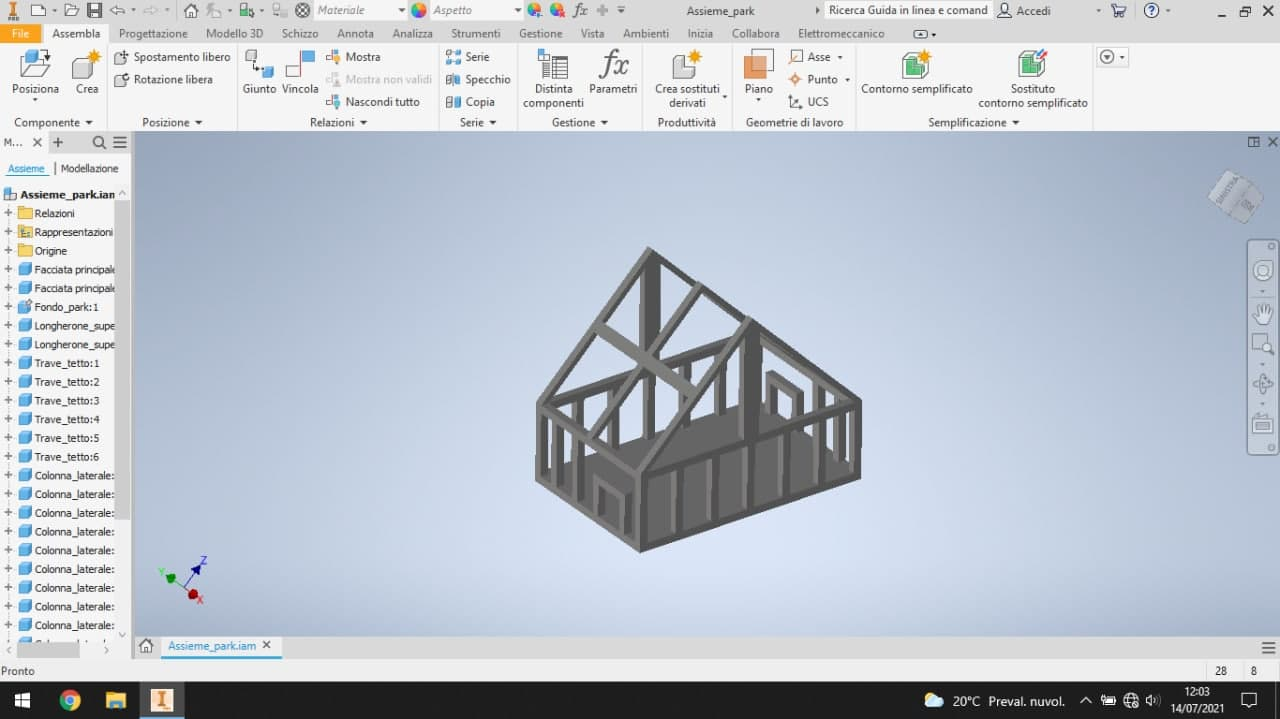
\includegraphics[width=\textwidth]{modello_1}
		\caption{Modello vista 1}
		\label{modello_1}
	\end{minipage}
	\vspace{0.5cm}
	\begin{minipage}[b]{.45\textwidth}
		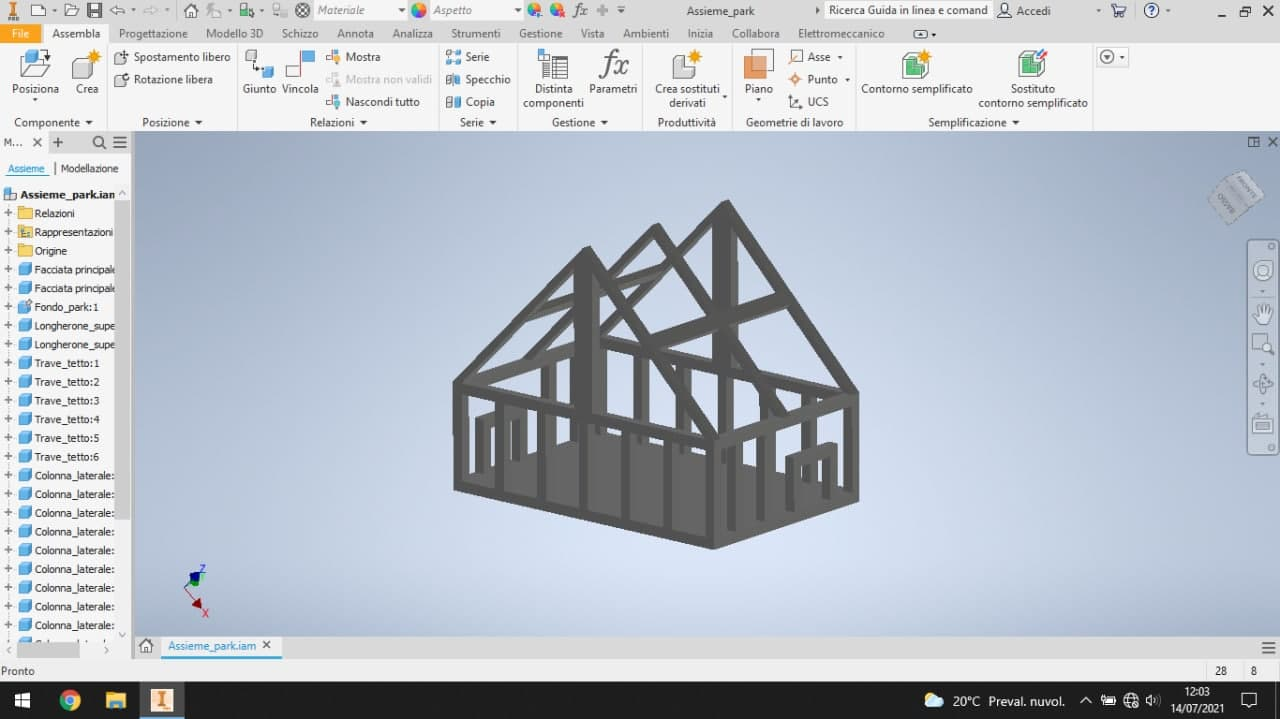
\includegraphics[width=\textwidth]{modello_2}
		\caption{Modello vista 2}
		\label{modello_2}
	\end{minipage}
	\begin{minipage}[b]{.45\textwidth}
		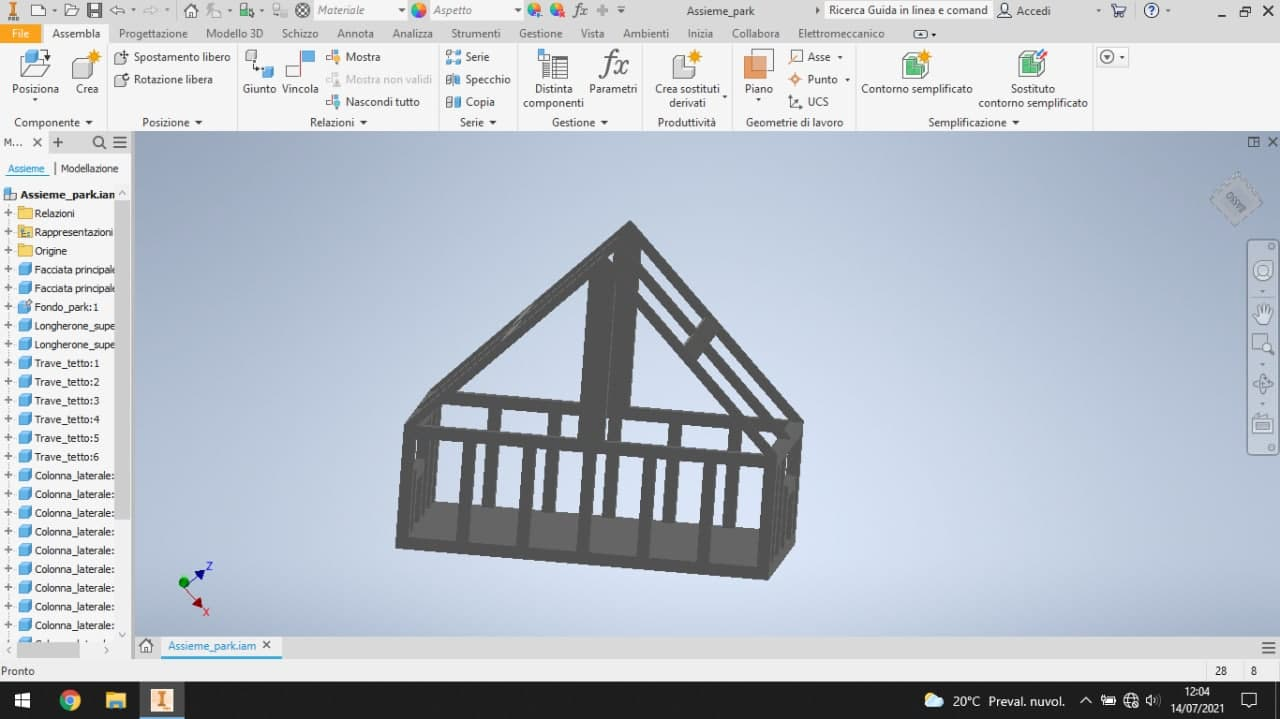
\includegraphics[width=\textwidth]{modello_3}
		\caption{Modello vista 3}
		\label{modello_3}
	\end{minipage}
\end{figure}

Il modello è composto da:
\begin{itemize}
	\item 10 colonne laterali;
	\item 2 facciate principali;
	\item 1 pavimentazione;
	\item 4 traverse del tetto;
	\item 2 sostegni per il tetto;
	\item 6 travi del tetto;
\end{itemize}
Le immagini relative ai piani di progettazione sono allegate alla relazione.

\chapter{Software}
\section{Web Application}
La gestione del parcheggio avviene mediante con architettura three tier. Il presentation layer è composto da una applicazione web che si occuperà di gestire gli input dell'utente per le prenotazioni e visualizzare le informazioni riguardanti il parcheggio o lo stato della prenotazione.
L'application layer si occupa di fornire tutte le funzionalità necessarie all'interfaccia grafica, mentre il data layer si occupa dell'interazione con la base di dati che conterrà tutte le informazioni relative alle prenotazioni e riguardanti il sistema fisico del parcheggio.
\newline Abbiamo optato per la combinazione di tre tecnologie software molto utilizzate negli ultimi anni:
\begin{itemize}
	\item \textbf{Angular 11} per gestire il frontend;
	\item \textbf{Django} per fornire i servizi necessari mediante delle API REST;
	\item \textbf{Oracle MySQL} come database management system;
\end{itemize}
\section{Front End - Angular}
Abbiamo deciso di adottare Angular nella sua versione 11, innanzitutto per imparare ad utilizzare un framework innovativo partendo da 0. Inoltre questo framework è sempre più utilizzato dalle case di sviluppo software odierne, incentivate sopratutto dal supporto di Google. \newline
Angular con la sua struttura modulare ed alla sua facile scalabilità permette di sviluppare software di qualità e prestazionale in modo relativamente semplice.
Questo framework open source è scritto in Typescript e permette uno sviluppo di applicazioni web su qualsiasi piattaforma e l'utilizzo dei servizi da ogni tipo di device. \newline
In combinazione con Angular di base abbiamo anche integrato il framework di markup Bootstrap 4.0, per rendere l'applicazione anche completamente responsive e gradevole nel suo aspetto. \newline
L'applicazione è strutturata nel seguente modo:
\newpage
\subsection{Home page}
La schermata principale conterrà alla prima visita due bottoni, uno per visualizzare le informazioni riguardanti l'ambiente del parcheggio ed un altro per poter effettuare la prenotazione.
\begin{figure}[H]
    \centering
    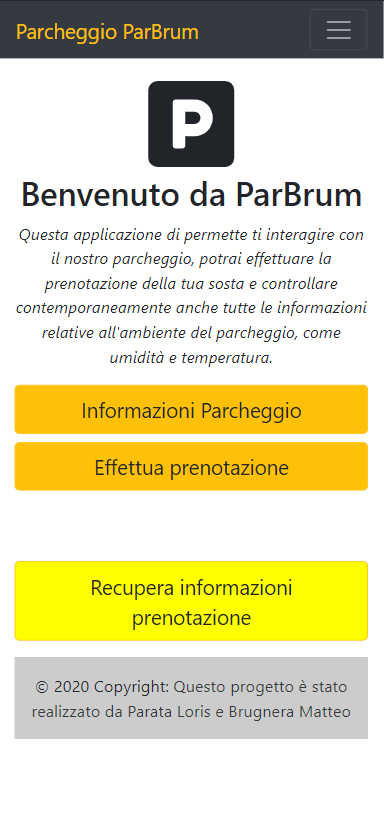
\includegraphics[width=0.25\textwidth]{home_page.png}
    \caption{Home Page ParBrum}
    \label{fig:homePage}
\end{figure}
\subsection{Informazioni del parcheggio}
L'utente potrà in ogni istante informarsi sulle condizioni meteo riguardanti il parcheggio, inoltre potrà verificare i valori relativi alla temperatura e all'umidità presente all'interno della struttura. L'utente potrà anche verificare l'eventuale numero di parcheggi liberi in quel determinato istante all'interno del parcheggio.
\begin{figure}[H]
    \centering
    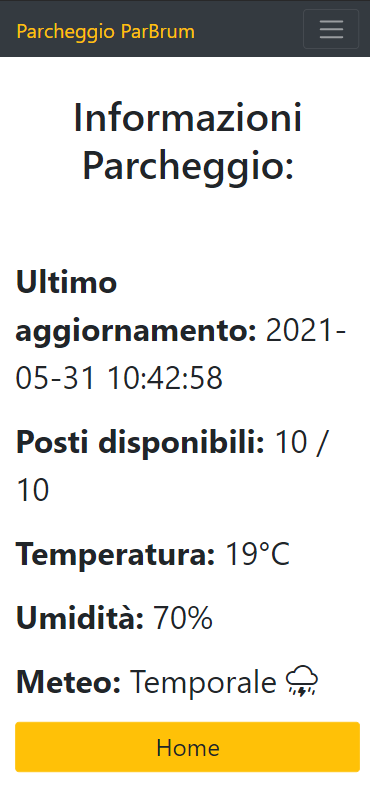
\includegraphics[width=0.25\textwidth]{info_parcheggio.png}
    \caption{Schermata "Informazioni Parcheggio" }
    \label{fig:infoParcheggio}
\end{figure}

\subsubsection{Condizioni meteo}
Le condizioni meteo non verranno calcolate direttamente dal sistema parcheggio, ma effettuiamo una richiesta ad un API esterna fornita da \textbf{OpenWeatherMap} a cui ci siamo registrati. Date le coordinate geografiche ci restituisce tutte le informazioni riguardanti il meteo del luogo richiesto in tempo reale.
\begin{figure}[H]
    \centering
    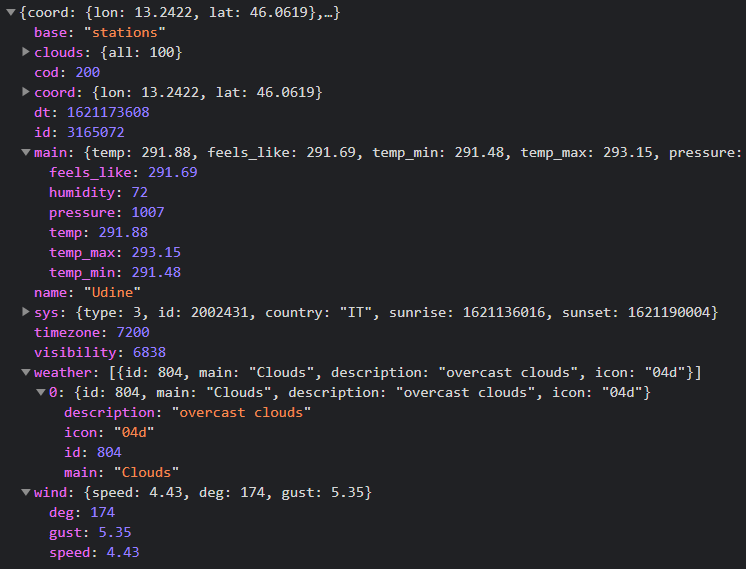
\includegraphics[width=0.55\textwidth]{weatherMap}
    \caption{Json servizio WeatherMap}
    \label{fig:jsonWeatherMap}
\end{figure}

\subsection{Richiesta di prenotazione}
L'utente potrà decidere di effettuare una richiesta di prenotazione per una determinata data cliccando sul bottone \textbf{Effettua Prenotazione}. \newline
Comparirà una schermata in cui dovrà inserire i dati necessari alla prenotazione, come Nome, Cognome, Email e Data di prenotazione. Una volta effettuata la richiesta il sistema verificherà la disponibilità di un posto nella data selezionata. Nel caso di esito positivo l'utente riceverà una notifica di conferma e verrà reindirizzato su una schermata contenente le informazioni riguardante la prenotazione.
\begin{figure}[H]
    \centering
    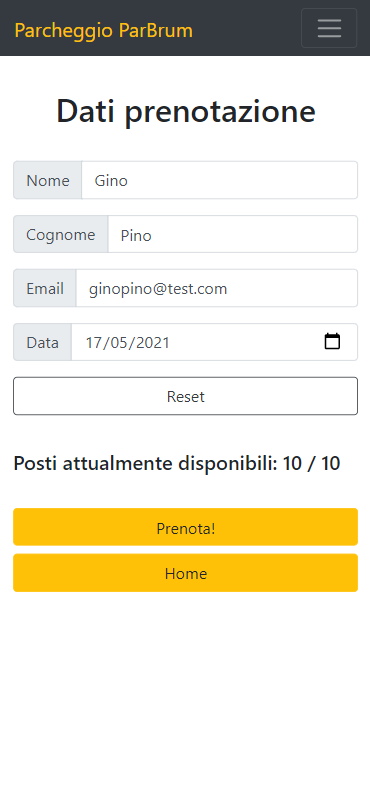
\includegraphics[width=0.25\textwidth]{prenotazione.png}
    \caption{Schermata "Richiesta Prenotazione"}
    \label{fig:richiestaPrenotazione}
\end{figure}
\subsubsection{Email di Conferma}
E' stata implementata anche una funzionalità aggiuntiva che nel momento in cui viene creata una prenotazione si andrà a generare una email contenente un riepilogo dei dati ed il codice QR generato dal sistema, in modo da poterlo utilizzare in alternativa alla sezione dedicata dell'applicazione web.
\begin{figure}[H]
	\centering
	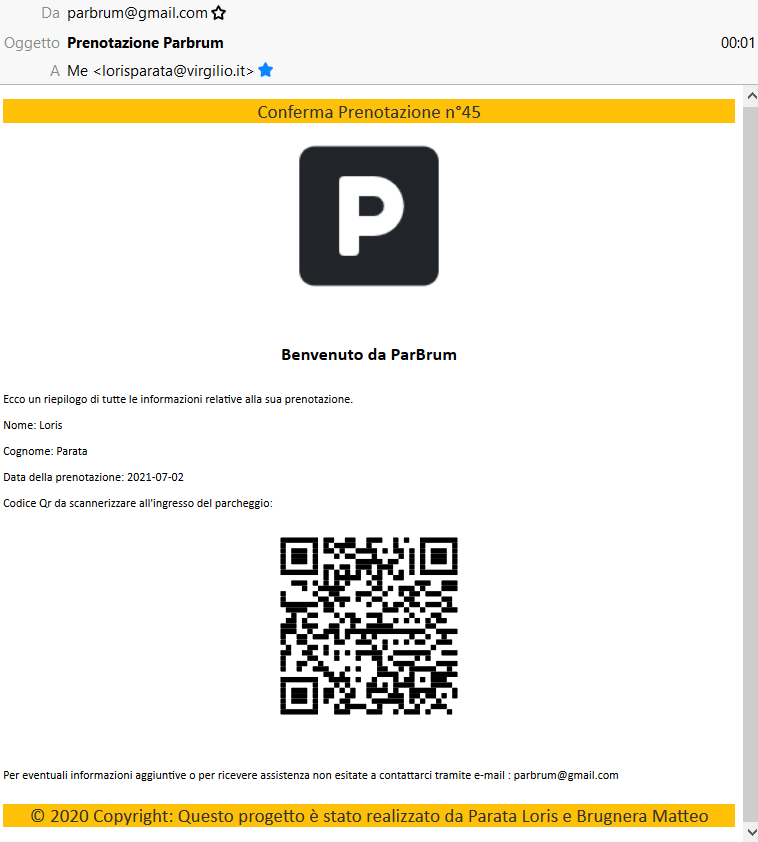
\includegraphics[width=0.45\textwidth]{figure/email_parbrum.PNG}
	\caption{Esempio email di conferma della prenotazione }
	\label{fig:conferma_prenotazione}
\end{figure}

\subsection{Prenotazione}
Questa schermata dell'applicazione conterrà tutte le informazioni riguardanti la prenotazione inseriti durante la fase di Richiesta di prenotazione, ed inoltre conterrà anche un QrCode che permetterà all'utente di accedere fisicamente al parcheggio. Questo QrCode verrà letto da una camera, verificato e successivamente permetterà all'utente di accedere al parcheggio. \newline
\begin{figure}[H]
    \centering
    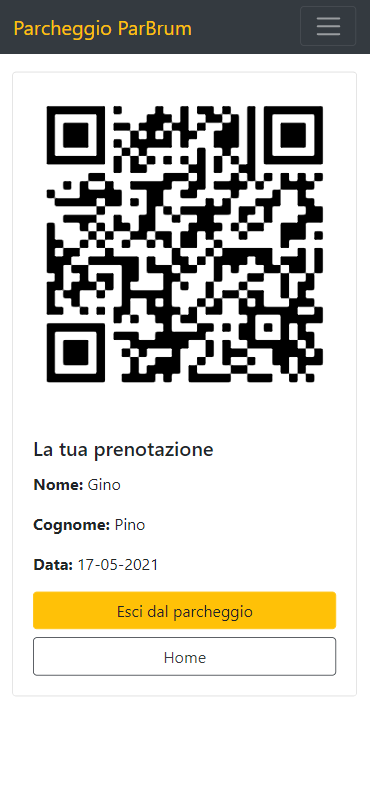
\includegraphics[width=0.25\textwidth]{prenotazione_effettuata.png}
    \caption{Schermata "Prenotazione"}
    \label{fig:prenotazione}
\end{figure}
Nella schermata è presente anche il bottone che permetterà all'utente di richiedere al sistema di uscire facendo aprire la sbarra.

\subsubsection{Recupero della prenotazione}
E' stata implementata anche una pagina che permette all'utente di recuperare i dati riguardanti una determinata prenotazione. In questo modo può accedere al servizio anche da un dispositivo differente, questo è possibile mediante un form. Le informazioni richieste sono il numero di prenotazione e la data corrispondente alla stessa, l'applicazione va a verificare i dati e rimanda l'utente alla pagina \textbf{Prenotazione} contenente i dati della prenotazione richiesta.
\newpage
\section{Back End - Django}
Per il backend abbiamo deciso di utilizzare Django, un framework scritto in Python. Esso è strutturato in modo tale da interagire un database MySQL e di fornire i servizi REST necessari al sistema di gestione del parcheggio. Tutti i servizi sono forniti mediante delle chiamate HTTP che restituiscono i dati richiesti sottoforma di JSON. Nel caso si tratti di chiamate che alterano lo stato del parcheggio, come la richiesta di uscire da esso, verranno restituiti dei JSON contenenti l'esito delle richieste.

\subsection{Models}
Il framework Django ci permette di creare dei modelli, paragonabili alle classi, che permettono di modellare il nostro sistema e le entità con cui andremo ad interagire. In base a come vengono definiti i dati, il framework stesso si occuperà di creare le tabelle definite all'interno del codice. Ogni classe corrisponde ad una determinata tabella, di cui definiamo i vari attributi e le loro caratteristiche, le chiavi primarie e le chiavi esterne che definiscono le relazioni tra le tabelle.
\begin{figure}[H]
    \centering
    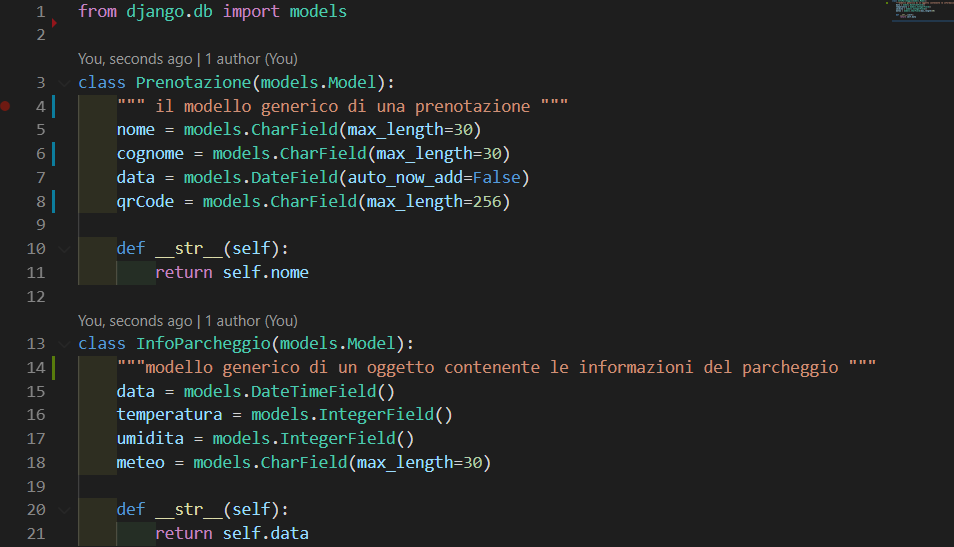
\includegraphics[width=0.75\textwidth]{models_py.png}
    \caption{Models backend }
    \label{fig:modelsBackend}
\end{figure}

\subsection{Views}
Questo framework ci permette di creare la logica applicativa dal punto di vista del backend mediante delle viste. Le viste sono un meccanismo del tipo "Request - Response", vengono richiamate tramite un URL specifico stabilito nel file urls.py. Ogni vista permette di attivare delle specifiche funzioni da noi definite e all'interno delle funzioni è possibile anche richiamare funzioni esterne o funzioni definite all'interno della logica del server. Questo sistema ci permette di riutilizzare il codice. Di specifico abbiamo utilizzato le \textbf{RedirectView} che ci permettono di interagire con le funzioni mediante delle chiamate HTTP.
\begin{figure}[H]
    \centering
	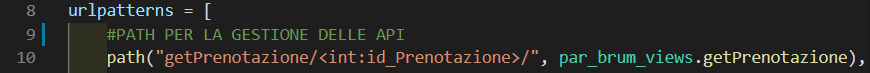
\includegraphics[width=0.75\textwidth]{urls_py.png}
    \caption{Urls backend}
    \label{fig:urlsBackend}
	\vspace{0.5cm}
   	 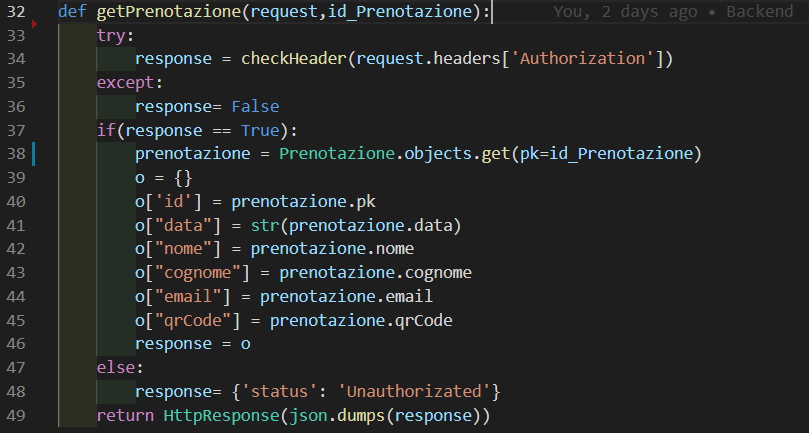
\includegraphics[width=0.75\textwidth]{views_py.png}
    \caption{Views backend}
    \label{fig:viewsBackend}
\end{figure}

\subsubsection{QrCode}
Il qrCode viene generato utilizzando la libreria \textbf{PyQrcode} a cui forniamo alcuni dati relativi alla prenotazione in maniera tale da renderli univoci per ogni prenotazione. Componiamo una stringa utilizzando id, nome, cognome e data della prenotazione.
A questa stringa applichiamo una funzione di Hash MD5 in modo da aumentare la confidenzialità dei dati. La stringa hashata verrà utilizzata per generare il QrCode che verrà memorizzato sottoforma di SVG sul server e la sua posizione nel campo apposito QrCode.

\begin{figure}[H]
    \centering
    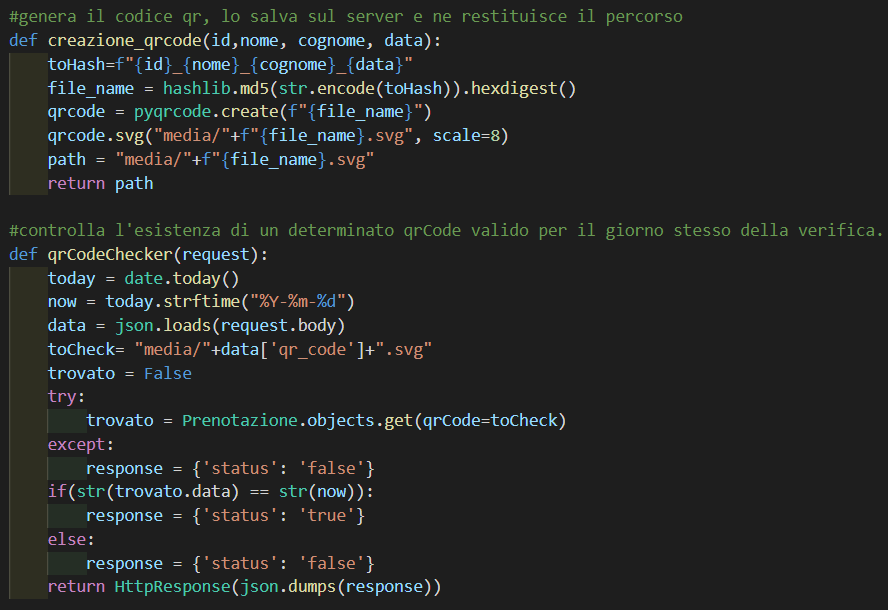
\includegraphics[width=0.75\textwidth]{qr_py.png}
    \caption{QrCode Backend ParBrum}
    \label{fig:qrCode Backend}
\end{figure}
Utilizzeremo la stessa stringa hashata per effettuare la convalida della prenotazione nel momento della lettura del qrCode da parte della camera.

\subsection{ JWT JSON Web Tokens}
Il JSON Web Token (JWT) è uno standard open (RFC 7519) che definisce uno schema in formato JSON per lo scambio di informazioni tra vari servizi.
Il token generato può essere firmato (con una chiave segreta che solo chi genera il token conosce) tramite l’algoritmo di HMAC, oppure utilizzando una coppia di chiavi (pubblica / privata) utilizzando gli standard RSA o ECDSA.
I JWT sono molto utilizzati per autenticare le richieste nei Web Services e nei meccanismi di autenticazione OAuth 2.0 dove il client invia una richiesta di autenticazione al server, il server genera un token firmato e lo restituisce al client che, da quel momento in poi, lo utilizzerà per autenticare le successive richieste.

\begin{figure}[H]
    \centering
    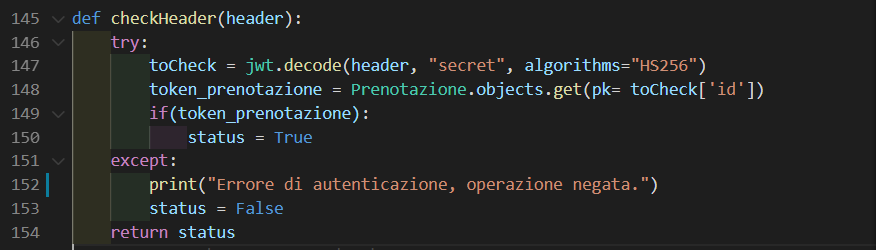
\includegraphics[width=0.75\textwidth]{jwt_py.png}
    \caption{JWT ParBrum}
    \label{fig:jwtBackend}
\end{figure}

Noi abbiamo abbiamo implementato questo standard per autenticare le richieste riguardanti la visualizzazione delle informazioni della prenotazione effettuata e nella fase di richiesta di uscita, andando a verificare chi effettivamente effettua la richiesta. L'autenticazione della richiesta avviene analizzando l'header della richiesta HTTP configurato a livello di front-end. Abbiamo installato la libreria \textbf{PyJWT} apposita per Python.

\chapter{Hardware}
Dal punto di vista hardware abbiamo utilizzato un Raspberry che gestisce il display LCD, i sensori e la mobilità del tetto. Inoltre abbiamo utilizzato anche un altro Raspberry Pi in combo con un microcontrollore Arduino, che si occupano dell'identificazione degli utenti tramite cam Pi con la conseguente gestione degli accessi alla struttura.
\section{Raspberry e Arduino}
L’apertura della sbarra d'accesso al parcheggio è stata effettuata tramite l’utilizzo di un Raspberry Pi in combinazione con un Arduino Uno. Questo microcontrollore è collegato a due led (uno rosso e uno verde), un micro servo sg90 e un buzzer.
L’utilizzo della scheda Arduino avviene tramite il protocollo pyFirmata.
Infatti, è stato caricato lo sketch StandardFirmata all’interno dell’Arduino, in modo tale da non utilizzare il suo IDE e la programmazione a basso livello della scheda, che è stata sostituita dal linguaggio di programmazione Python. In questo modo non serve più caricare e compilare altri sketch su Arduino.
\subsection{PyFirmata}
Il firmware pyFirmata è un protocollo per la comunicazione su porta seriale fra microcontrollore e computer host. E' possibile sfruttare questa protocollo andando a caricare uno sketch predefinito sul microcontrollore Arduino e di gestire la comunicazione con il dispositivo direttamente ad alto livello mediante delle librerie apposite utilizzabili in Python. Questo pacchetto dà l’accesso completo ai pin presenti su Arduino, con conseguente possibilità di lettura e scrittura di su un qualsiasi pin presente.
\begin{figure}[H]
	\centering
	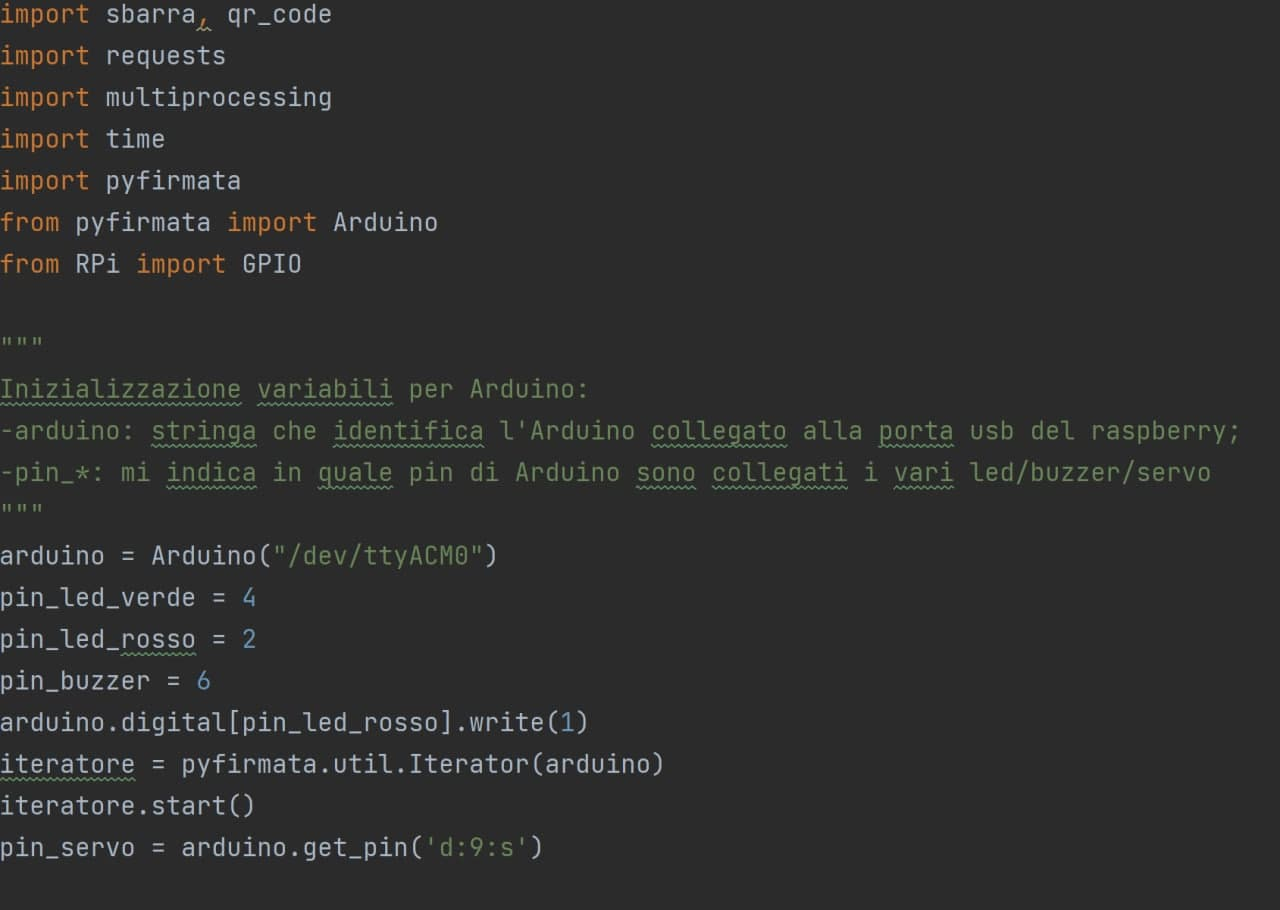
\includegraphics[width=0.5\textwidth]{figure/ini_arduino.jpg}
	\caption{Inizializzazione Arduino con PyFirmata}
	\label{pyfirmata}
\end{figure}
Nella parte di script presente nella figura \ref{pyfirmata} vengono importate le librerie necessarie all'utilizzo dei dispositivi. Inoltre vengono inizializzati tutti gli attuatori, assegnando i vari pin su cui verranno effettuate le scritture dei valori da parte delle funzioni.

\subsection{Apertura sbarra}
\begin{figure}[H]
	\centering
	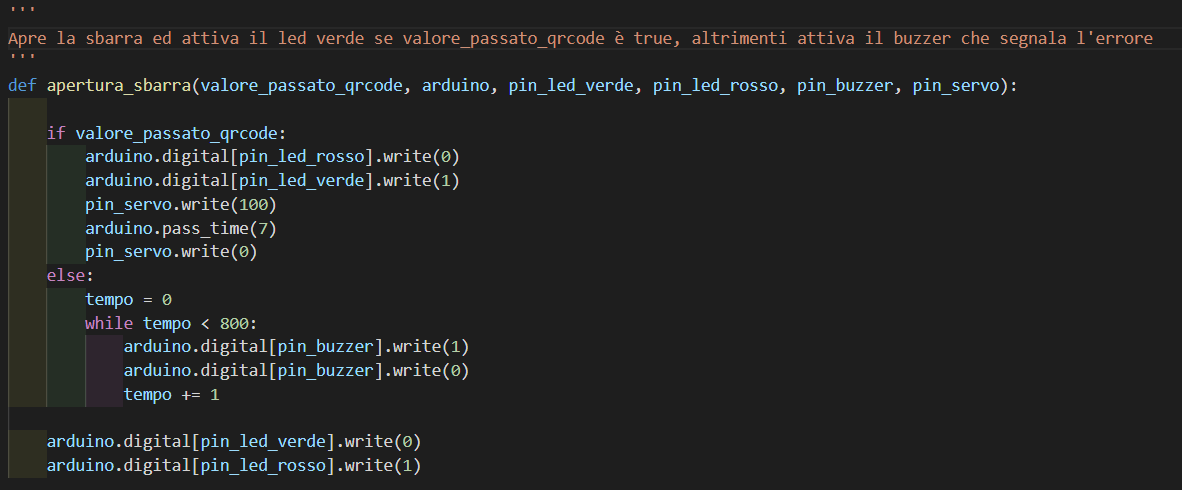
\includegraphics[width=0.75\textwidth]{figure/apertura_sbarra}
	\caption{Script apertura della sbarra}
	\label{apertura_sbarra}
\end{figure}
Lo script presente in figura \ref{apertura_sbarra} viene utilizzato per l’apertura della sbarra mediante l'attivazione del servomotore corrispondente per l’ingresso e l’uscita dal parcheggio.
La funzione riceve in ingresso un valore booleano, risultato ottenuto dalla scansione e verifica del qrcode. Nel caso di esito positivo, allora viene mandato il comando ad Arduino per aprire la sbarra e richiuderla dopo 7 secondi.
Se il riconoscimento fallisce viene attivato il buzzer che emetterà un suono.
\subsubsection{Lettura e controllo dati contenuti nel QrCode}
\begin{figure}[H]
	\centering
	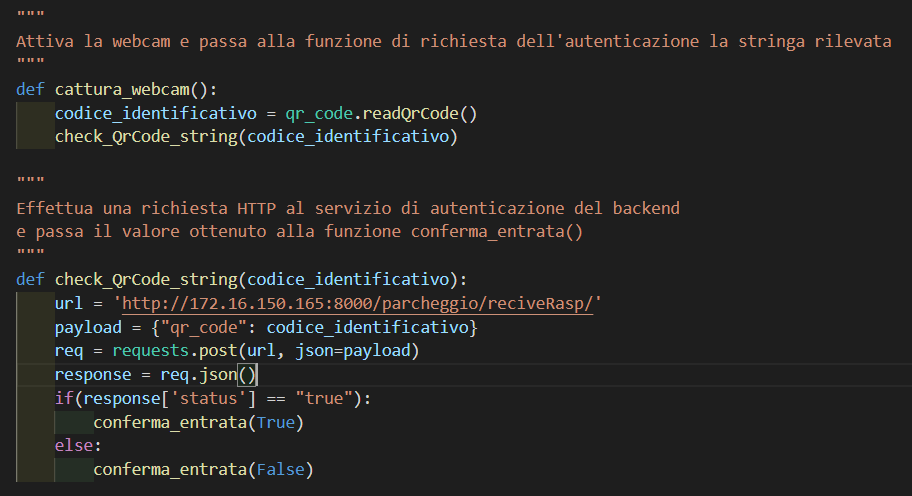
\includegraphics[width=0.75\textwidth]{figure/cattura_qrCode.jpg}
	\caption{Cattura del codice QrCode}
	\label{catturaQr}
\end{figure}
La funzione \textbf{cattura\_webcam()} della figura \ref{catturaQr} richiama la funzione \textbf{readQrCode()} che attiva la camera che legge i QrCode e restituisce la stringa letta. 
Questa stringa viene successivamente passata a \textbf{check\_QrCode\_string()} che invierà una richiesta al servizio responsabile dell'identificazione dell'utente. In base alla risposta del servizio verrà aperta o meno la sbarra.


\section{Raspberry}
Il secondo Raspberry Pi esegue lo script che gestisce le informazioni rilevate dai sensori, le invia alla base di dati e contemporaneamente le visualizza sullo schermo che a rotazione visualizza le informazioni e un messaggio di benvenuto. Inoltre lo script legge le informazioni integrative relative al meteo attuale dalla base di dati ed effettua una eventuale modifica sullo stato di apertura del tetto.

\subsubsection{RPi GPIO}
E' un pacchetto di librerie che permette di controllare i pin GPIO (general-purpose input/ouput) di Raspberry Pi. Con la conseguente possibilità di controllare moltissimi dispositivi come lcd, servi e sensori.
\begin{figure}[H]
	\centering
	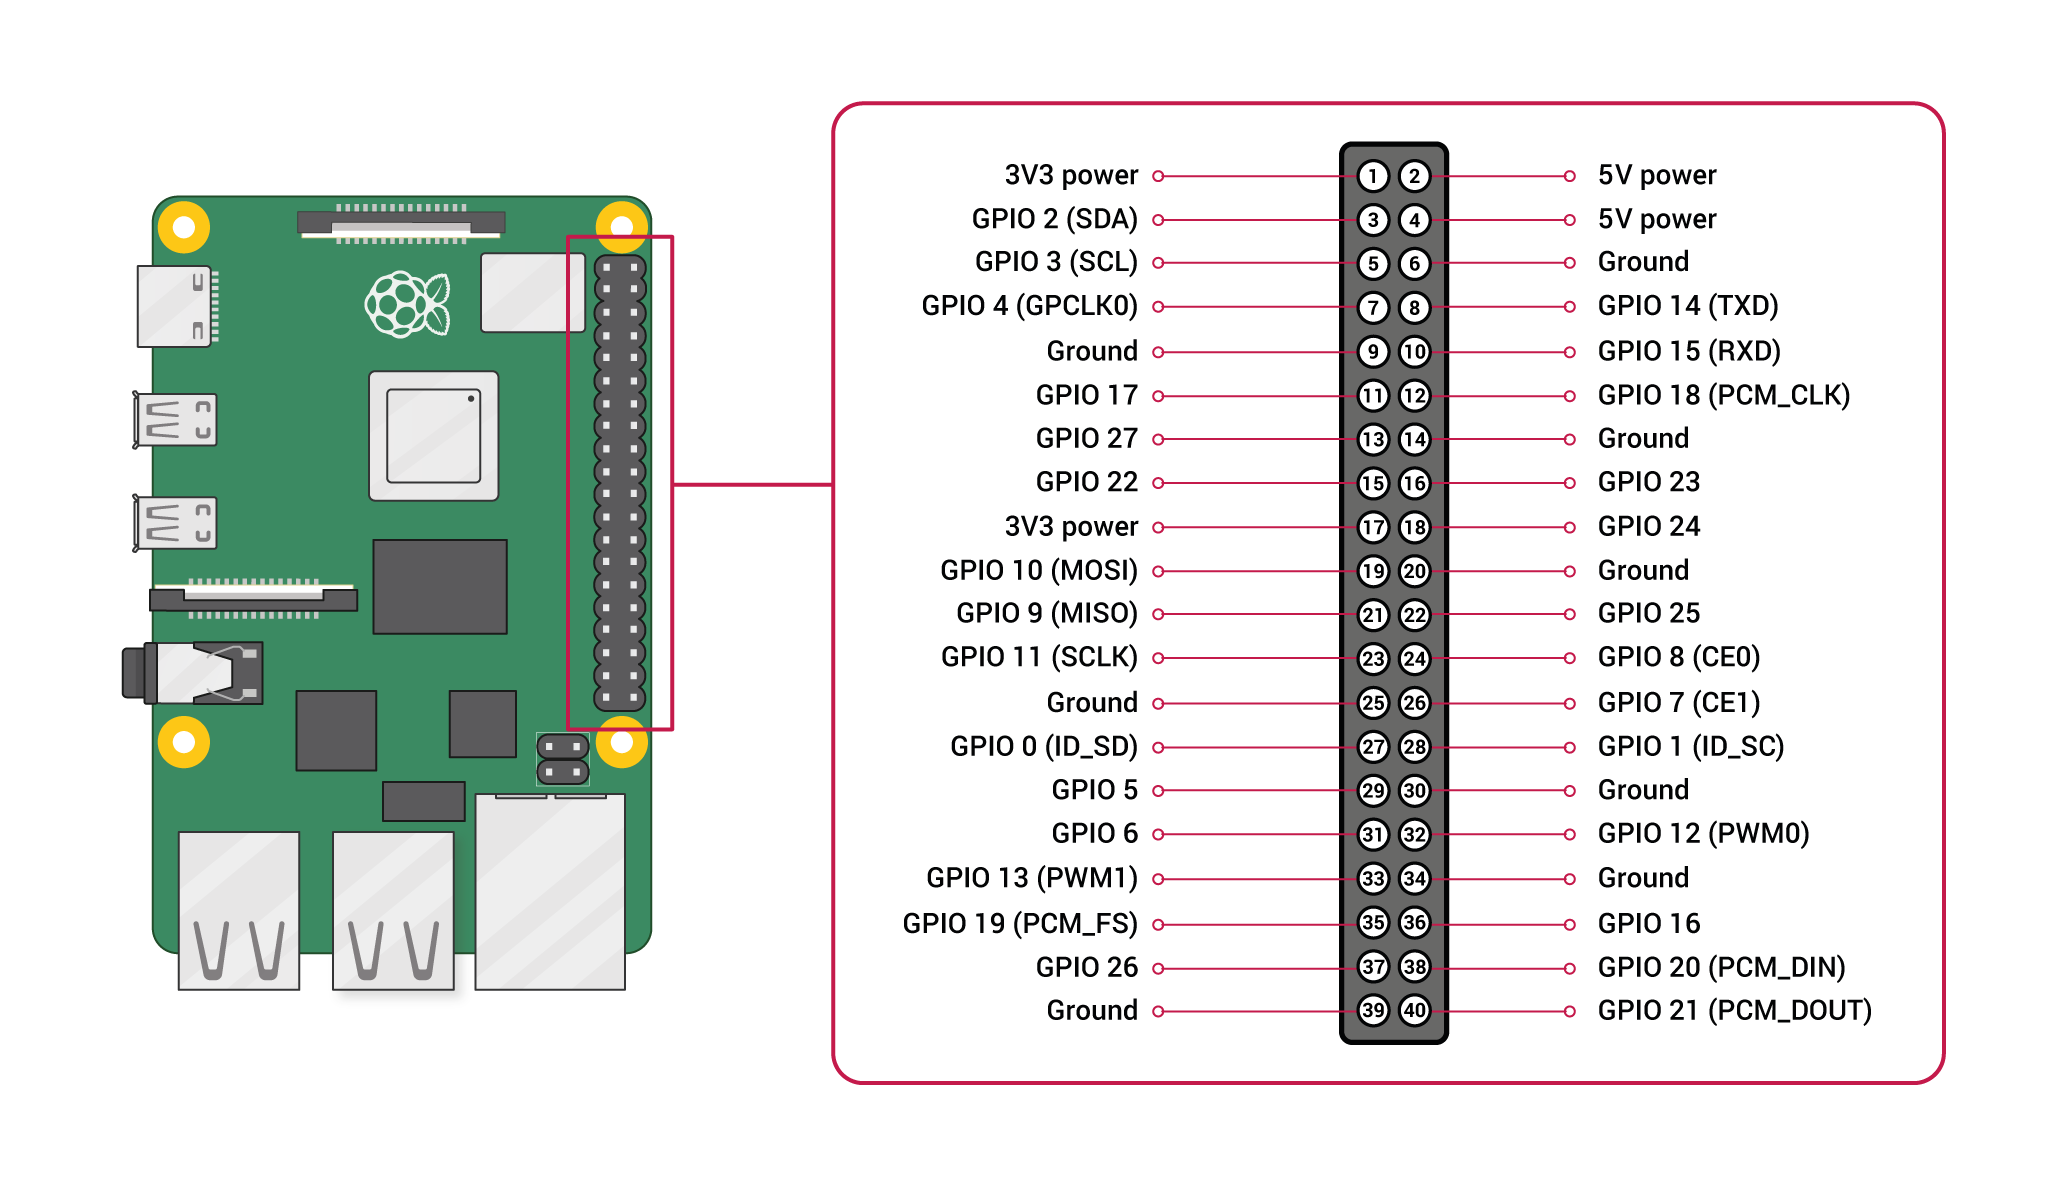
\includegraphics[width=0.99\textwidth]{figure/GPIO-Pinout-Diagram-2.png}
	\caption{Schema pin Raspberry Pi}
	\label{temp}
\end{figure}

\subsection{Calcolo della temperatura}
\begin{figure}[H]
	\centering
	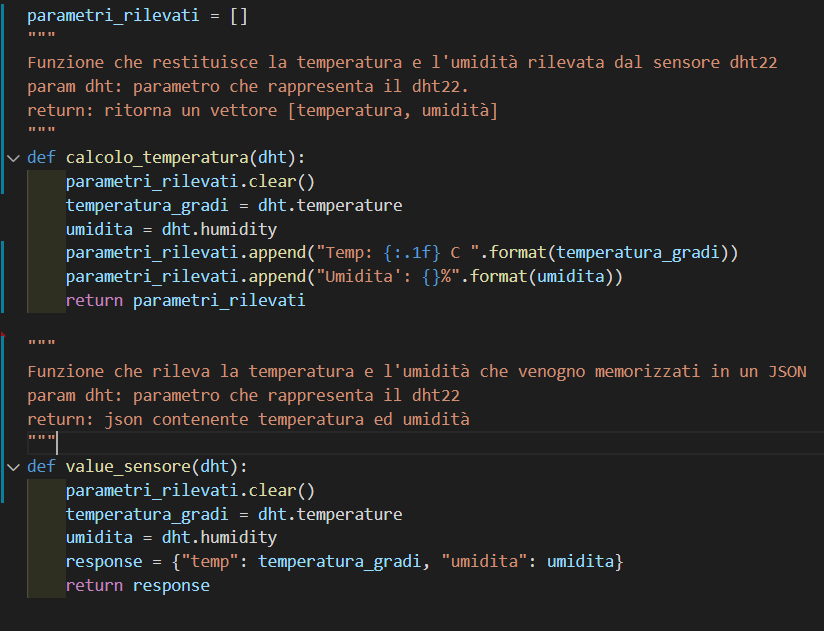
\includegraphics[width=0.75\textwidth]{temperatura_rasp}
	\caption{Funzione rilevazione temperatura e umidità}
	\label{temp}
\end{figure}
Lo script in figura \ref{temp} ha il compito di calcolare la temperatura e l’umidità tramite l’utilizzo del sensore dht22 e della libreria adafruit\_dht.
Sono state formulate due funzioni differenti per fare ciò:
\begin{itemize}
	\item 1. \textbf{calcolo\_temperatura()} si crea la stringa che verrà poi utilizzata dal programma incaricato a mostrare a display il risultato;
	\item 2. \textbf{value\_sensore()} i dati rilevati dal sensore vengono salvati in formato JSON. Questa funzione verrà richiamata per salvare all’interno del database tutte le rilevazioni effettuate per mantenere uno storico.
\end{itemize}

\subsection{Visualizzazione informazioni LCD}
\begin{figure}[H]
	\centering
	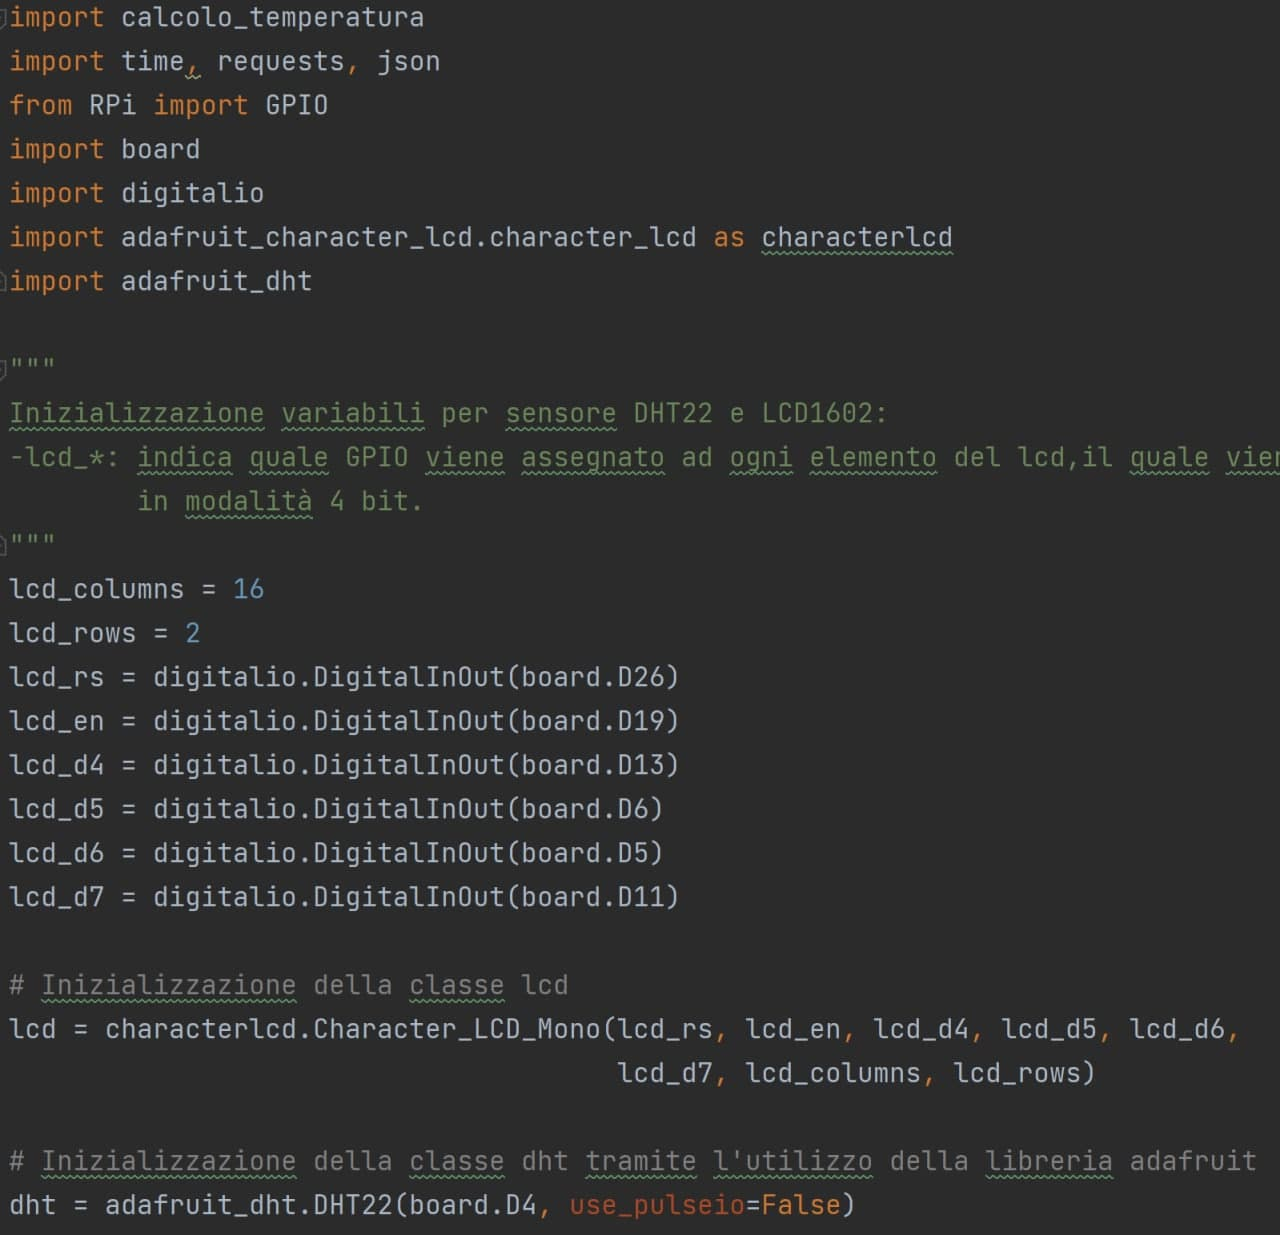
\includegraphics[width=0.65\textwidth]{lcd_1}
	\caption{Import librerie, inizializzazione LCD e DHT22 }
	\label{lcd_in}
\end{figure}
Nell'immagine \ref{lcd_in} si può notare come viene importato lo script “\textbf{calcolo\_temperatura}”, che ci permette di ottenere i dati relativi alla temperatura utilizzando lo script analizzato nella figura \ref{temp}.
Utilizziamo le librerie \textbf{adafruit\_character} e \textbf{digitalio} per l’utilizzo del display, \textbf{adafruit\_dht} per l’utilizzo del sensore dht22 e per la gestione dei servomotori utilizziamo la libreria \textbf{GPIO}.
Nella seconda parte del codice viene inizializzato sia il DHT22 che l’LCD. Per quanto riguarda quest’ultimo, si indicano quante colonne e righe vengono utilizzate e subito dopo si elencano i pin occupati all’interno del Raspberry Pi, utilizzati per inviare i segnali al display.
\begin{figure}[H]
	\centering
	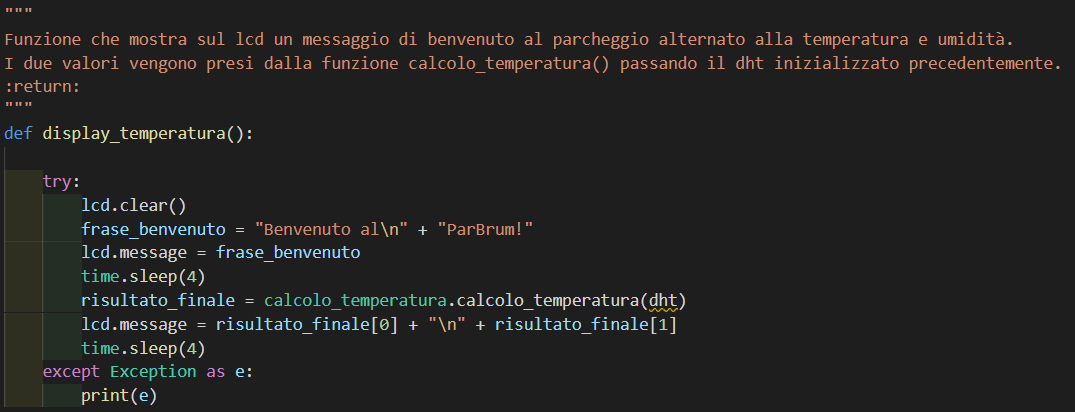
\includegraphics[width=0.75\textwidth]{lcd_2}
	\caption{Funzione che visualizza le informazioni sul display}
	\label{lcd_view}
\end{figure}
Nella figura \ref{lcd_view} è presente la funzione \textbf{display\_temperatura()}, che visualizza sullo schermo lcd un messaggio di benvenuto al parcheggio, seguito da una seconda schermata contenente tutte le informazione legate alla temperatura e all’umidità rilevante nel parcheggio.

\subsection{Controllo del meteo, temperatura e umidità}
\begin{figure}[H]
	\centering
	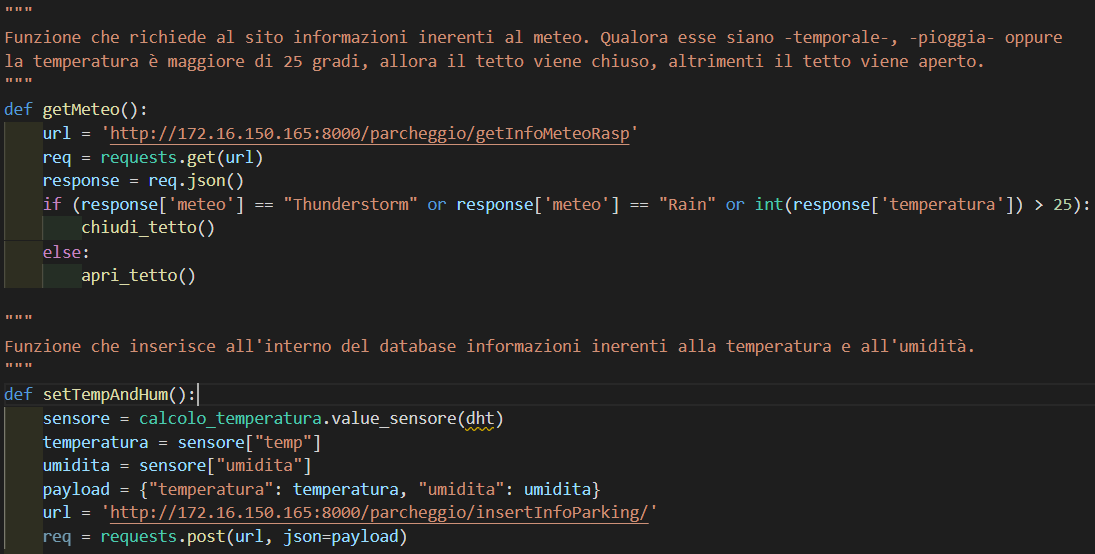
\includegraphics[width=0.75\textwidth]{figure/meteo_1.jpg}
	\caption{Funzione che verifica le condizioni meteo}
	\label{meteo_1}
\end{figure}

La funzione \textbf{getMeteo()} permette di reperire le informazioni legate alle condizioni meteo direttamente dalla base di dati del sistema parcheggio effettuando una richiesta all'API corrispondente.
\subsubsection{Inserimento informazioni sensori nel database}
La seconda funzione in figura \ref{meteo_1} \textbf{setTempAndHum()} permette di inserire all’interno del database le informazioni relative al temperatura e umidità rilevate dal raspberry. La funzione invia in formato JSON le informazioni mediante una richiesta http del tipo POST ad una API apposita del sistema parcheggio, in modo tale da creare uno storico.
In particolare, qualora il contenuto del JSON restituito nel campo \textbf{['meteo']} risulti essere uguale a 'thunderstorm', 'rain' oppure la temperatura è maggiore di 25 gradi, allora viene chiamata la funzione \textbf{chiudi\_tetto()}, in caso contrario viene chiamata la procedura \textbf{apri\_tetto()}.

\subsection{Apertura e chiusura del tetto}

\begin{figure}[H]
	\centering
	\begin{minipage}[b]{.5\textwidth}
		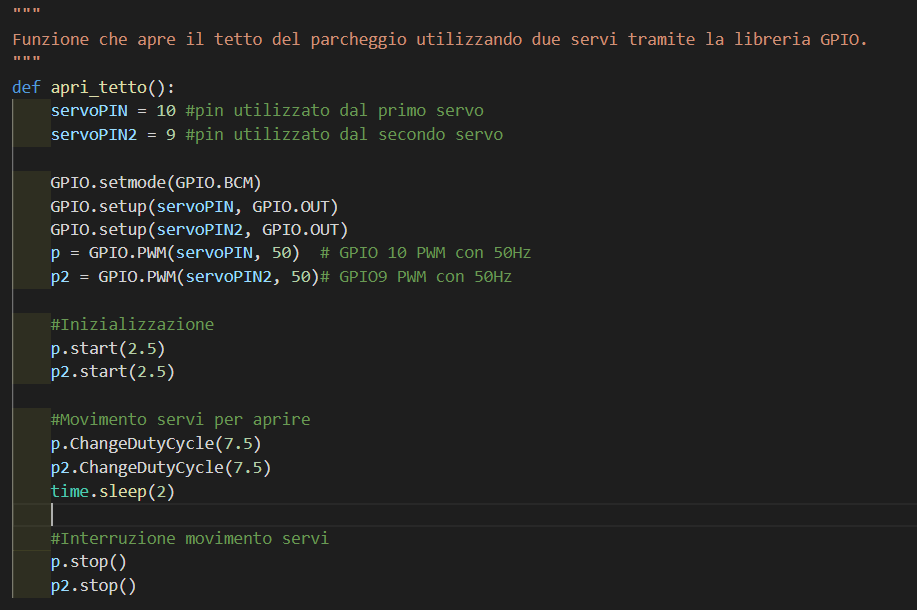
\includegraphics[width=\textwidth]{servo_1}
		\caption{Funzione apertura tetto}
		\label{servo_1}
	\end{minipage}
	\begin{minipage}[b]{.485\textwidth}
	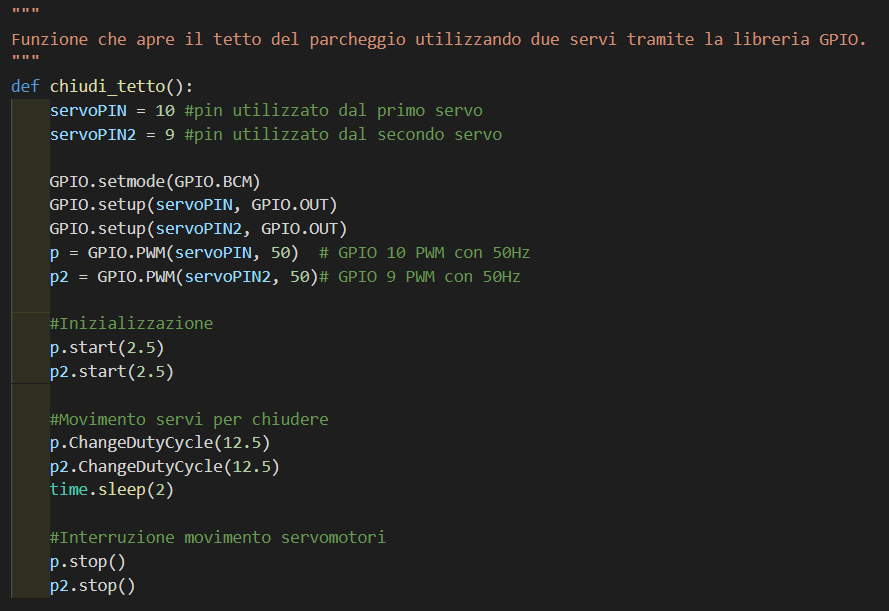
\includegraphics[width=\textwidth]{servo_2}
	\caption{Funzione chiusura tetto}
	\label{servo_2}
	\end{minipage}
\end{figure}

Le due funzioni che troviamo nella figura \ref{servo_1} e \ref{servo_2} servono per aprire e chiudere il tetto del parcheggio.
Inizialmente vengono indicati i pin di riferimento per l’utilizzo dei due servo motori. Dopo aver fatto il setup(), a cui vengono passati i pin di input e output per inizializzarli, viene utilizzata la funzione \textbf{ChangeDutyCycle()}, a cui viene passato l'impulso adatto per ottenere l'angolo di rotazione desiderato. Questo permette di effettuare i movimenti riguardanti l’apertura e la chiusura del tetto. Al termine della funzione, i due servo motori vengono fermati grazie alla chiamata \textbf{stop()}.

\subsection{Main}
Tutte le funzioni descritte precedentemente vengono richiamate in un ciclo while, che presenta all'interno un tempo di attesa arbitrario, per esempio 60 secondi, in modo da eseguirle ciclicamente.

\subsection{Uscita dal parcheggio}
L'uscita del parcheggio è effettuata mediante un piccolo Web server,in esecuzione sul Raspberry collegato alla sbarra d'ingresso, che mette a disposizione una API REST.  Quando viene richiamato il servizio viene eseguita la funzione \textbf{apertura\_sbarra()} della figura \ref{apertura_sbarra}. 
Questo servizio viene richiamato dall'applicazione lato client.

\begin{figure}[H]
	\centering
	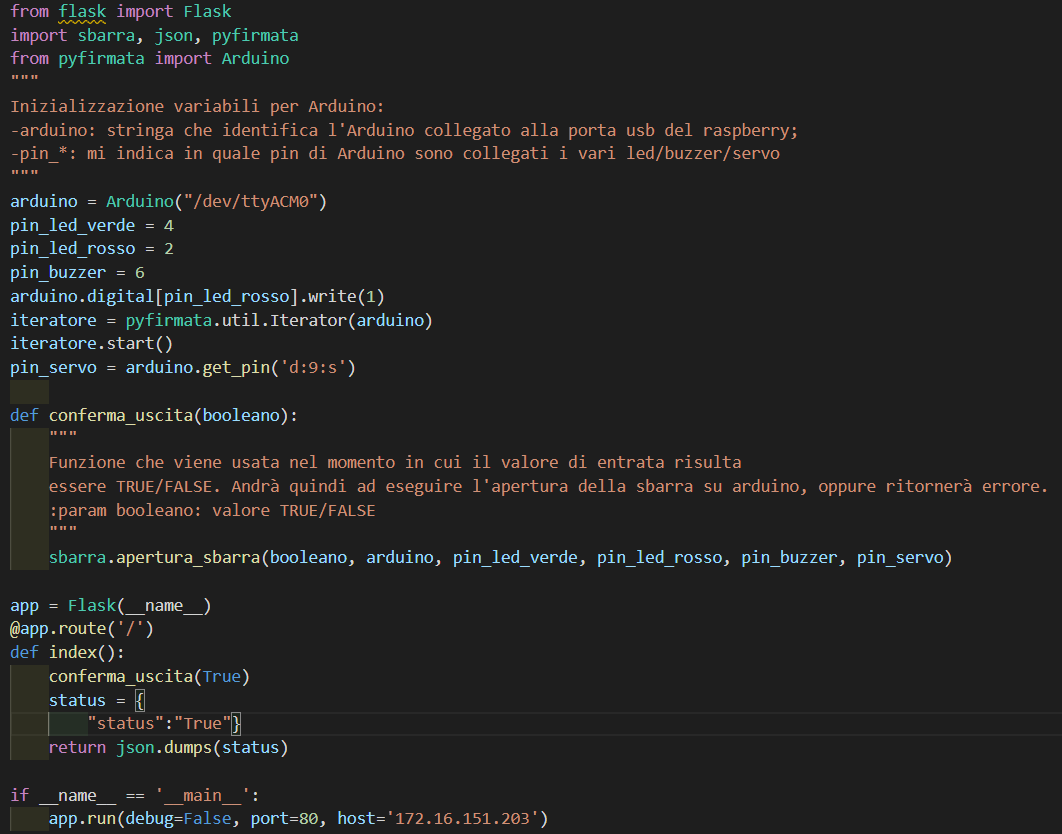
\includegraphics[width=0.75\textwidth]{figure/web_server}
	\caption{Web server che gestisce le richieste di uscita dal parcheggio}
	\label{parcheggio_uscita}
\end{figure}


\chapter{Conclusioni}
\section{Possibili sviluppi futuri}
Questo prototipo potrebbe essere sviluppato creando una rete di parcheggi appartenenti ad uno stesso ente, implementando di conseguenza una gestione dei vari parcheggi a livello di software amministrativo ed implementare la gestione degli utenti, in maniera tale da permettere anche uno storico delle varie prenotazioni effettuate nei vari parcheggi nel tempo. \newline
Si potrebbe anche implementare un sistema di riconoscimento delle targhe che permetterebbe all'utente di evitare la scansione del codiceQR, mantenendolo soltanto come sistema alternativo di autenticazione. \newline
Nel caso in cui un'azienda volesse implementare questo sistema, rendendolo un servizio privato per gli utenti, sarebbe necessario implementare la gestione dei pagamenti in base al tempo trascorso all'interno del parcheggio.

\section{Informazioni conclusive}
Alleghiamo alla relazione del progetto tutto il codice scritto per la realizzazione e un video che ne visualizza il funzionamento completo.
\end{document}